\documentclass[pdf,mia,noFooter,slideColor,colorBG]{prosper}

\usepackage{amsmath}
%\usepackage{color}



\begin{document}

\title{Title}
\subtitle{Subtitles}
\author{Smurf}
\email{smurf@inra.fr}
\institution{INRA}

%\maketitle

\begin{slide}{}
\psline[linewidth=50pt,linecolor=white](-2,1.4)(10.3,1.4)
\rput[lb](2.5cm,0.4cm){\includegraphics[width=5cm]{Page1_top.eps}}
 \rput[lb](-0.3cm,-1.4cm){\includegraphics[width=10.5cm]{logoMIA19x2.eps}}
  \rput[lb](0.8cm,-4.8cm){Evaluation of the MIA Department -- October 2006}
 \rput[lb](-1.8cm,-5.2cm){\rotatebox[origin=c]{0}{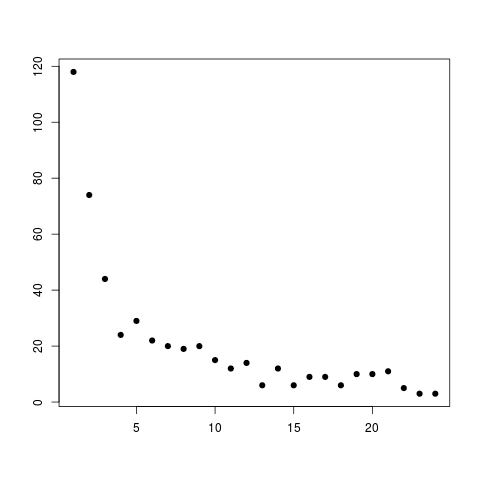
\includegraphics[width=2cm]{butterfly.eps}}}
\rput[lb](-2cm,-7.35cm){\includegraphics[width=13.7cm]{Page1_bottom.eps}}

  \rput[lb](0.5cm,-2.1cm){\Large\textbf{Statistics for Systems Biology}}
\end{slide}


%====================================
\begin{slide}{SSB group}
\begin{itemize}
\item 3 MIA units: Jouy, Paris, Evry
  
\item 30 scientists

\item Statistics for sequence analysis, microarray data, 3D-structure
  prediction, biological networks, etc.

\item blabla

\end{itemize}

\end{slide}
%====================================

%====================================
\begin{slide}{Two illustrations}
\begin{itemize}
\item Biological sequence analysis via HMM
  
% \begin{small}
%   \begin{equation*}
%     \frac{1}{\pi}=\sum_{n=0}^\infty \frac{(\frac{1}{4})_n(\frac{2}{4})_n(\frac{3}{4})_n}{n!^3}\bigl(2\sqrt{2}(1103+26390n)\bigr)\frac{1}{(99^2)^{2n+1}}
%   \end{equation*}
%   \end{small}

\item Statistical analysis of biological networks

\end{itemize}

\end{slide}
%====================================


%====================================
\begin{slide}{Sequence analysis via HMM}


\end{slide}
%====================================


%====================================
\begin{slide}{Statistics of networks}

\begin{itemize}
\item model for random graphs

\item significant structures in a biological network (motifs,
  diameter, etc.)

\end{itemize}


\end{slide}
%====================================




\end{document}
